%%%%%%%%%%%%%%%%%%%%%%%%%%%%%%%%%%%%%%%%%%%%%%%%%%%%%%%%%%%%%%%%%%%%%%%%%%%%%%%%

% Preamble

%%%%%%%%%%%%%%%%%%%%%%%%%%%%%%%%%%%%%%%%%%%%%%%%%%%%%%%%%%%%%%%%%%%%%%%%%%%%%%%%

% Page Settings
\documentclass[10pt]{report}
\usepackage[T1]{fontenc}
\usepackage[utf8]{inputenc}
\usepackage[letterpaper, margin=1in, left=1.5in]{geometry}

% Bibliography
\usepackage{biblatex}
\addbibresource{ref/thesis.bib}

% Packages
\usepackage{svg}
\usepackage{titlesec,hyperref,booktabs,relsize,setspace,float,verbatim,caption,subcaption,graphicx}
%\hypersetup{colorlinks=true,linkcolor=blue,urlcolor=blue,citecolor=blue}
\hypersetup{hidelinks}
\titleformat{\chapter}[hang]
{\normalfont\huge\bfseries}{\chaptertitlename\ \thechapter:}{1em}{}
\setcounter{tocdepth}{1}

% Formatting
\doublespacing{}
%\setlength{\textfloatsep}{30pt plus 2.0pt minus 4.0pt}

% Identification
\title{}
\author{Christopher T. Tastad}
\date{day month year}

\begin{document}

%%%%%%%%%%%%%%%%%%%%%%%%%%%%%%%%%%%%%%%%%%%%%%%%%%%%%%%%%%%%%%%%%%%%%%%%%%%%%%%%

% Introductory Material

%%%%%%%%%%%%%%%%%%%%%%%%%%%%%%%%%%%%%%%%%%%%%%%%%%%%%%%%%%%%%%%%%%%%%%%%%%%%%%%%

% Title Page
\thispagestyle{empty}
\begin{center}
    \vspace*{1cm}

    \Huge
    \textbf{Refactoring the\\Candidate Cancer Gene Database}

    \vspace{1cm}
    \Large
    A Thesis\\
    SUBMITTED TO THE FACULTY OF THE\\
    UNIVERSITY OF MINNESOTA\\
    BY\\

    \vspace{1.5cm}

    \LARGE
    \textbf{Christopher T. Tastad}

    \vspace{3cm}

    \Large
    IN PARTIAL FULFILLMENT OF THE REQUIREMENTS\\
    FOR THE DEGREE OF\\
    MASTER OF SCIENCE\\

    \vspace{1cm}

    Adviser: Timothy K. Starr, PhD\\

    [full month and year of degree conferral]

\end{center}

% Copyright Page
\newpage
\thispagestyle{empty}

MIT License

Copyright (c) 2019 University of Minnesota

Permission is hereby granted, free of charge, to any person obtaining a copy of this software and associated documentation files (the ``Software''), to deal in the Software without restriction, including without limitation the rights to use, copy, modify, merge, publish, distribute, sublicense, and/or sell copies of the Software, and to permit persons to whom the Software is furnished to do so, subject to the following conditions:

The above copyright notice and this permission notice shall be included in all copies or substantial portions of the Software.

THE SOFTWARE IS PROVIDED ``AS IS'', WITHOUT WARRANTY OF ANY KIND, EXPRESS OR IMPLIED, INCLUDING BUT NOT LIMITED TO THE WARRANTIES OF MERCHANTABILITY, FITNESS FOR A PARTICULAR PURPOSE AND NONINFRINGEMENT\@. IN NO EVENT SHALL THE AUTHORS OR COPYRIGHT HOLDERS BE LIABLE FOR ANY CLAIM, DAMAGES OR OTHER LIABILITY, WHETHER IN AN ACTION OF CONTRACT, TORT OR OTHERWISE, ARISING FROM, OUT OF OR IN CONNECTION WITH THE SOFTWARE OR THE USE OR OTHER DEALINGS IN THE SOFTWARE\@.

% Acknowledgements
\newpage
\pagenumbering{roman}

acknowledgements

% Dedication
\newpage

dedication

% Abstract
\newpage

\section{Abstract}
Maintenance and upgrades are a fundamental requirement of any software-based tool, and the resources within the field of Bioinformatics are no exception. Too often, the combination of using self-taught programmers who are typically trained Biologists along with the broader lack of a software development ecosystem can propagate elevated degrees of software entropy, also known as technical debt. It is then a fair assumption to say that this level of entropy is higher than in fields which more consistently employ the skills of professional developers. Here, we present the case of the Candidate Cancer Gene Database (CCGD, https://z.umn.edu/ccgd) as a minor instance of taking advantage of an upgrade cycle in an attempt to service some of this technical debt. The goals of this project ultimately strived to achieve the implementation of a new, core framework at the base of the data integration backend as well as a more modern and simplified web front-end. In all, this represented a complete rebuild of the application while preserving the existing conceptual implementation. Our work served to establish a new application with greater structural simplicity, improved resource use, and, most relevant, a code base which will be easier to maintain and upgrade in the future.

\tableofcontents
\addcontentsline{toc}{chapter}{List of Tables}
\listoftables
\addcontentsline{toc}{chapter}{List of Figures}
\listoffigures

\newpage

\pagenumbering{arabic}

%%%%%%%%%%%%%%%%%%%%%%%%%%%%%%%%%%%%%%%%%%%%%%%%%%%%%%%%%%%%%%%%%%%%%%%%%%%%%%%%

% Introduction

%%%%%%%%%%%%%%%%%%%%%%%%%%%%%%%%%%%%%%%%%%%%%%%%%%%%%%%%%%%%%%%%%%%%%%%%%%%%%%%%


\chapter{Introduction}
In many ways, the field of Bioinformatics exists as the result of a problem rather than a discovery, as with other scientific fields. The nature of the challenges have evolved from a growth in the composition of primary data and a lacking compensatory set of technical skills to evaluate it. With the bottle neck that exists at the center of this problem, previously simple notions of collating, analyzing, and visualizing results no longer scale. As a result, a measurable area of focus is not just in the novel discovery of Biological relevance but in advancement of those engineer tools that offer new or dynamic means to solve old problems with new solutions. Further, the crossover of Biological and technical expertise has offered, at times, a cluttered approach to implementing these solutions resulting in less than desirable engineering.

All while this dynamic has developed in the world of Biology, the technology has rapidly improved. A pillar of the field's advances is in the area of web technologies, which now offer frameworks and tools that both accomplish more while requiring less of their developers. The classical paradigm of the web has evolved from the LAMP stack (Linux, Apache, MySQL, PHP) to improved frameworks such as advanced JavaScript, CSS3, and HTML5 that lay the foundation for modern and flexible web applications. These improvements have served to enhance the functionality of applications along with creating a reformed development process that is more intuitive, more accessible, and, ultimately, more powerful. These advances offer specific utility to the sciences, and following a comparable progress in application bears consideration.

While the implementation of new models typically applies to future work, it is essential to look back at opportunities to improve past engineering with updated models through the process of code refactoring. At a basic level, refactoring is simply restructuring or rewriting the content of a codebase while retaining the functionality of that service. This can serve many purposes that all aim to accomplish some range of improvements to the backend design, architecture, or performance. Within many engineering goals, this process offers access to items that address routine maintainability to wholesale upgrade. At times, this may not just be preferable but essential in the scope of scheduled updates and general obsolescence, making it a critical process in the scope of software development.

In this work, we present a small but emblematic case that illustrates these shifting paradigms. With these incremental changeovers, no mater the impact, the field takes on a new character in the management of its growing data challenges. The CCGD as a concept set out to tackle some of the original problems of filtering handling large quantities of data. We expand on this by re-implementing the same achievement through a modern application.

%Gene screens in cancer bio~\cite{Clark2019}

%Cancer gene screening is a hallmark case for this exploration as it lives at the nexus of being an area of high impact research and a process that can produce a deluge of raw data. In tandem, the state of web front ends has advanced in a manner that more completely allows~\cite{10.1093/nar/gkz1161}

%%%%%%%%%%%%%%%%%%%%%%%%%%%%%%%%%%%%%%%%%%%%%%%%%%%%%%%%%%%%%%%%%%%%%%%%%%%%%%%%

% Body

%%%%%%%%%%%%%%%%%%%%%%%%%%%%%%%%%%%%%%%%%%%%%%%%%%%%%%%%%%%%%%%%%%%%%%%%%%%%%%%%

\chapter{Body}

\section{Methods}

\subsection{Project Requirements}
This project's goal was ultimately to upgrade the existing CCGD\@. In setting out to do this, we established several requirements that took into consideration the opportunity to seize a routine set of server transitions to implement improved functionality. Specifically, the central output of the service should be retained in the eyes of the end user. Beyond this, attempting to fully reconstruct the backend provided for significant improvements (see Table~\ref{table:projectReqs}). These goals more broadly were: upgrade the existing server build to RHEL 7; rewrite web interface in a more modern framework; streamline the central table construction process using Rshiny; implement improved ability to manipulate table and web content by product owner (Tim Starr); employ improved software development best practices; generally seek opportunities for codebase and resource utilization improvements. Ultimately, all of these taken together were intended to serve some form of modernization and simplification.

\begin{table}[H]
    \caption{Project Requirements}\label{table:projectReqs}
    \relsize{-2}
    \addtolength\tabcolsep{-0.2em}
    \begin{tabular}{llllp{7cm}}
        \toprule
        &Feature&Goal&Framework&Description\\
        \midrule
        1&server OS&upgrade server OS&RHEL7&Transition of architecture for public server host. This is required by University OIT due to end of life schedule for RHEL6.\\
        \midrule
        2&web front-end&rewrite web interface&Rmarkdown&Improvements to the web interface written in a modern, simplified language. This improved access to content creation and allowed for automation in front-end rendering.\\
        \midrule
        3&table build&rewrite table build&Rshiny&Rshiny offered a dramatic improvement to replace the existing process by merging the table build back-end with a modern web display of the app interface.\\
        \midrule
        4&content update&improved admin controls&BASH/R&Old app version confined some content controls to app author, limiting ability to make contributions by product owner (Tim Starr).\\
        \midrule
        5&version control&implement best practices&git/docs&No version control was used in the original development of the app. This and other documentation practices were expanded in the rewrite.\\
        \midrule
        6&multiple&resource improvements&codebase&Due to the lack of some best practices, there were many opportunities to make impactful resource improvements.\\
        \bottomrule
    \end{tabular}
    \addtolength\tabcolsep{+0.2em}
    \relsize{+2}
\end{table}

\subsection{Server Setup}
At it's core, the OS transition from RHEL 6 to 7 was the original project requirement that spurred this work. Existing hosting for the CCGD was owned by university OIT who established an end of life date for the current server OS\@. As a result, the bulk of core architecture implementation followed a narrow prescription for what was termed a ``Fully Managed'' RHEL7 install as detailed by the OIT-LPT Public-Docs~\cite{oitOITLPTPublicDocsThis}. Contrary to the implications of this installation name, a Fully Managed administration carried a mixture of privileges and management roles that were shared between OIT and our group. This was accomplished by leveraging a chef admin paradigm that allowed limited sudo privileges within the hosted ecosystem. Importantly, items that extend from the core of server administration such as virtual machine creation, backups, and core security were handled by OIT\@. This left our group with the more focused task of administering exclusively our application.

\subsection{Web Framework}
The upgraded build of the CCGD employed a completely different front-end architecture centralized around R web services environment. Built with dynamic modularity and data portability in mind, the Rmarkdown framework offers the ability to render several independent markdown files into a unified website. We applied this feature set to produce our general site structure and content as it allowed for a massive simplification in web design. While following the existing site map, we recreated the raw content of the existing application as independent markdown files. Within the Rmarkdown format guide. The keystone feature of the Rmarkdown framework that allows for this unified rendering is the use of a YAML configuration header (see Figure~\ref{fig:siteYaml}). The \texttt{rmarkdown::render\_site} function leverages this configuration file to align and sequentially render content and styling in tandem for a complete site map [citeme rmarkdown docs]. Additionally, individual markdown pages employ this same configuration paradigm for page-specific parameters and formatting guidelines (see Figure~\ref{fig:pageHeader}).

\begin{figure}[H]
    \center{}
    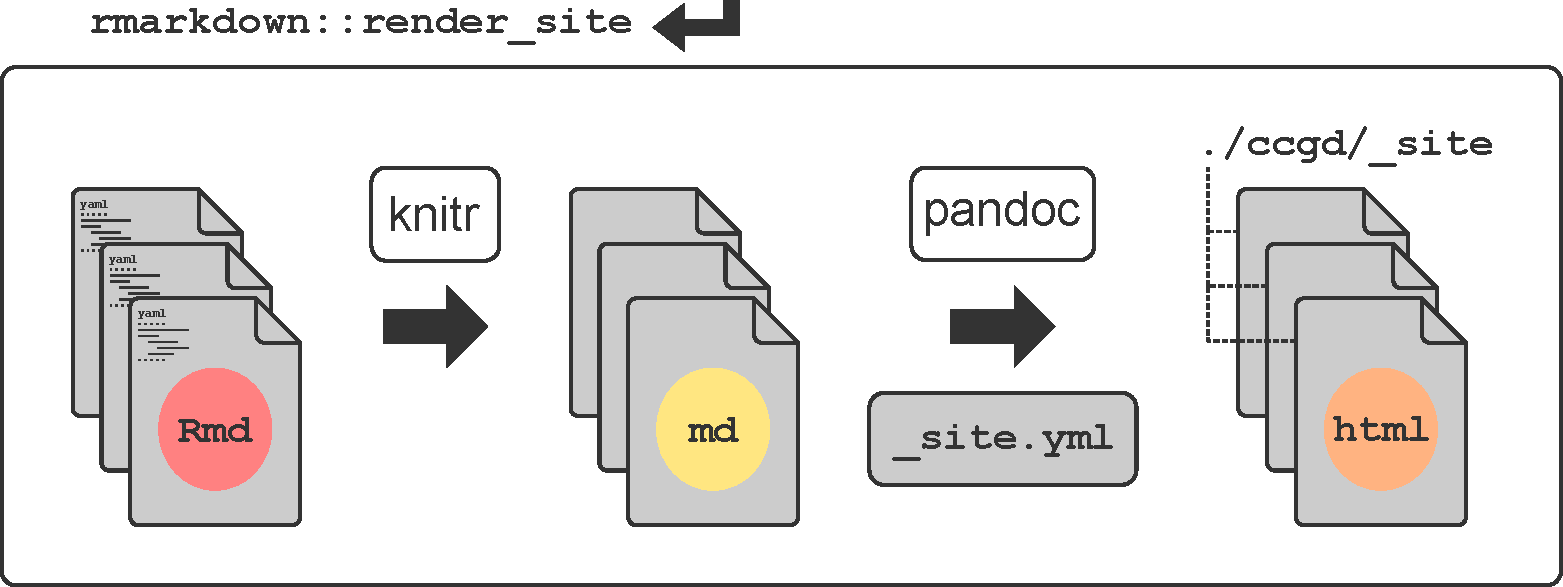
\includegraphics[width=0.8\textwidth]{fig/rmarkdown_flow.pdf}
    \caption[Rmarkdown Rendering Flow]{\textbf{Rmarkdown Rendering Flow} The core web framework was created using a stitch process composed of two document conversion steps, which are both contained in the single \texttt{rmarkdown::render\_site} command. These two transformations are done by the R-specific knitr package and then the open-source Pandoc tool. The first phase holds less relevance in particular as its role is to execute R code chunks, of which there are few in our page content. The markdown output from this step is seamlessly injected into a Pandoc conversion which offers a large variety in document output. Specific to our case, the Pandoc conversion paired with a companion YAML configuration file allows for multi-document markdown-to-html rendering which is assembled as a complete site stack. As a single process, this function generates an integrated, modern web front-end from content written in a light-weight syntax with almost none of the typical complexity of full-scale web page creation.}\label{fig:renderFlow}
\end{figure}

responsive web design

An important distinction in summarizing the implementation of web framework is to point out that the Rshiny app, which contains the gene table, is assembled and hosted as a function separate from the general site rendering. More specifically to the web design, the shiny app is hosted at the common public repository \href{https://ctastad.shinyapps.io/table_app/}{\texttt{shinyapps.io}} and rendered in an inline iframe on the site search page. In the eyes of the user this presents a seamless transition, but the functional contrast permits for differential rendering between the two. This allows for the continuous integration of external sources that feed the table while eliminating the need to regularly render the static site content.

\begin{figure}
    \center{}
    \begin{subfigure}[t]{.3\textwidth}
        \center{}
        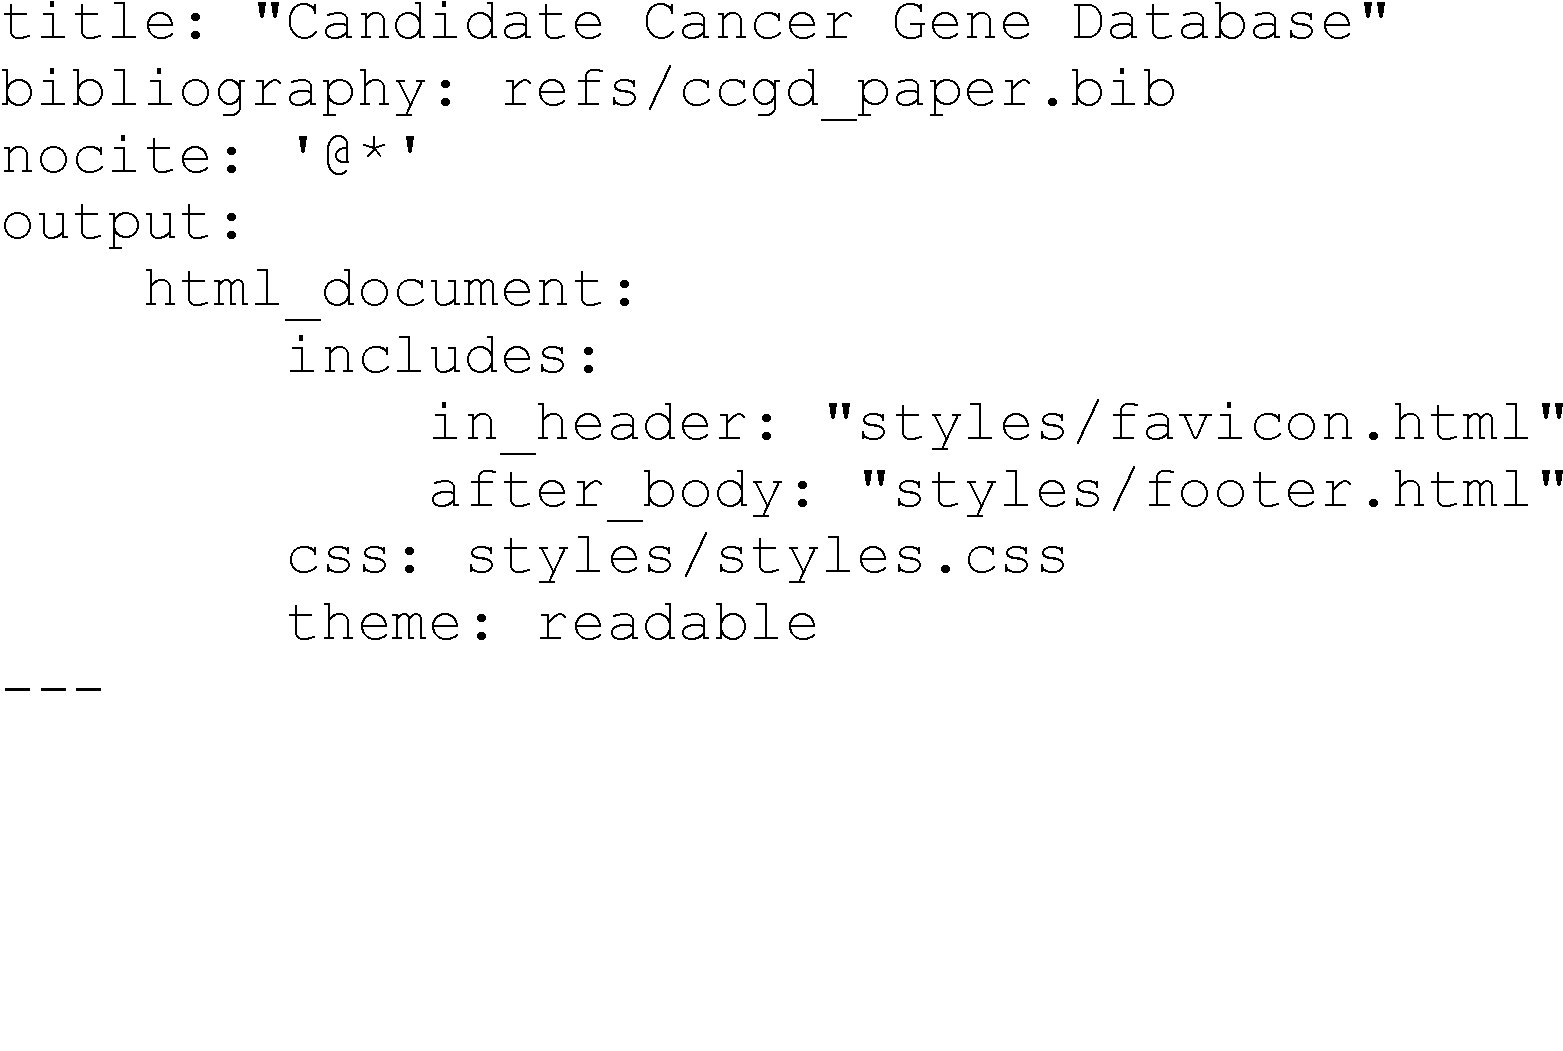
\includegraphics[width=\textwidth]{fig/page_header.pdf}
        \subcaption{index.Rmd individual page header}\label{fig:pageHeader}
    \end{subfigure}%
    \hspace{2em}
    \begin{subfigure}[t]{.3\textwidth}
        \center{}
        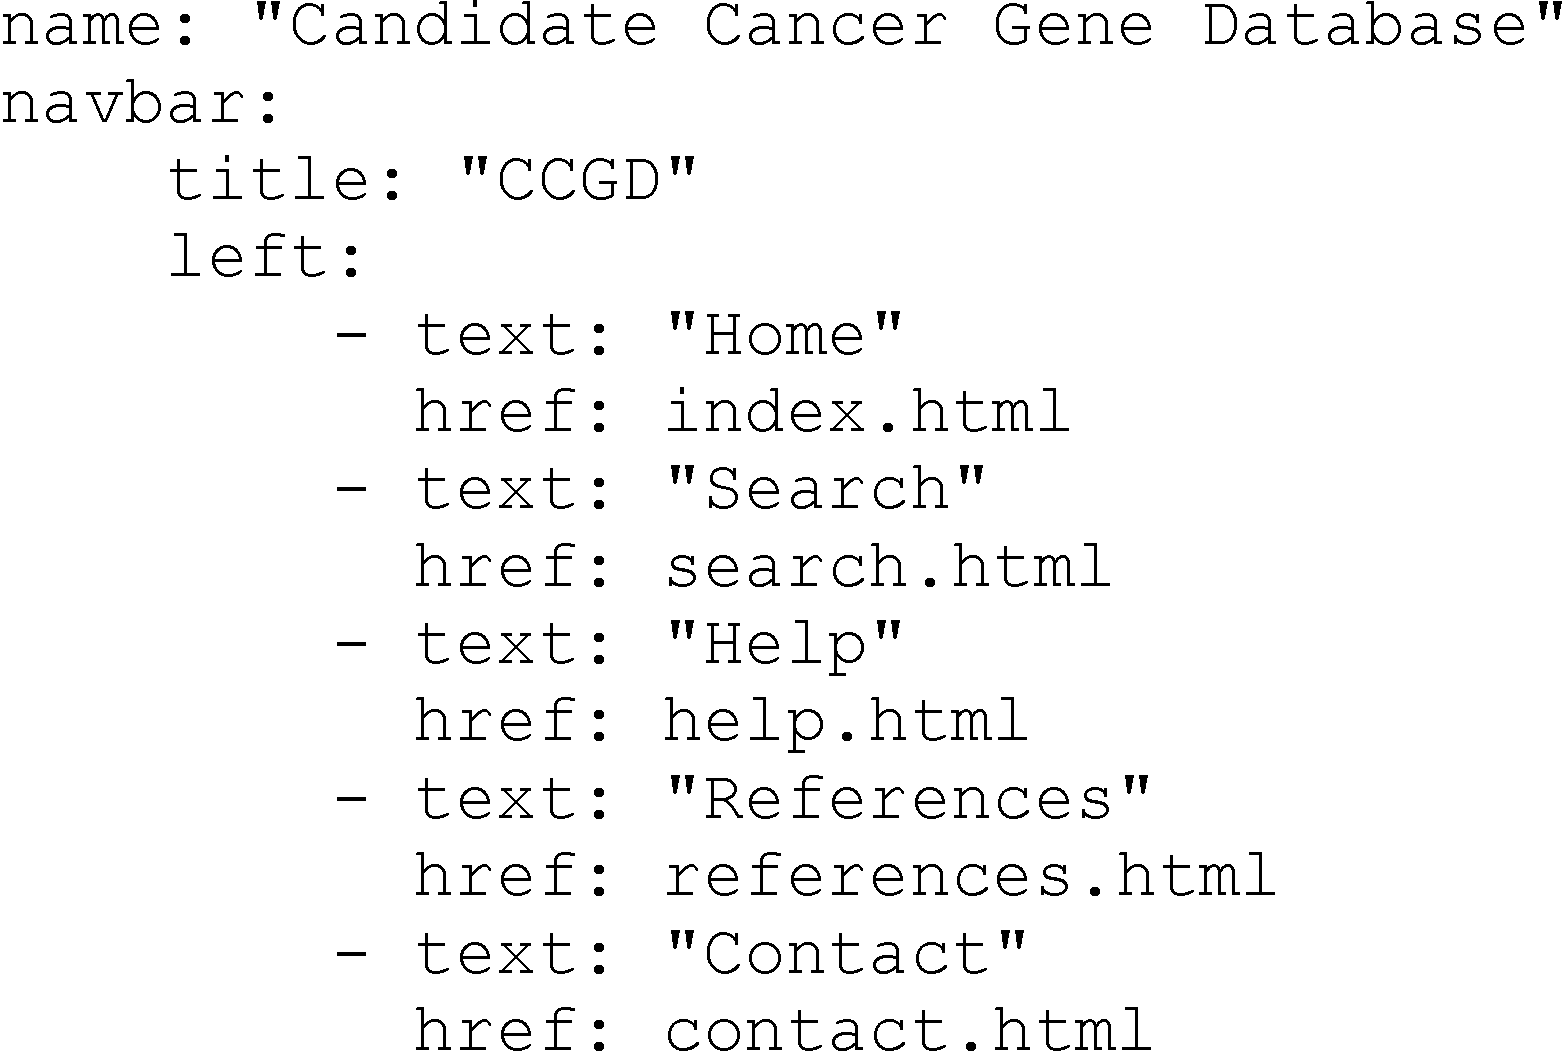
\includegraphics[width=\textwidth]{fig/site_header.pdf}
        \caption{\_site.yml: file for site assembly}\label{fig:siteYaml}
    \end{subfigure}
    \hspace{2em}
    \begin{subfigure}[t]{.2\textwidth}
        \center{}
        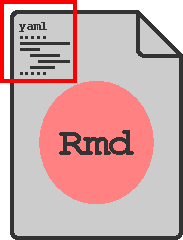
\includegraphics[width=0.8\textwidth]{fig/yaml_illustration.pdf}
        \caption{Illustration of yaml implementation}\label{fig:yamlIllust}
    \end{subfigure}
    \caption[YAML Configuration Segments]{\textbf{YAML Configuration Segments} Pictured above are the two forms of complete YAML configuration headers utilized in Rmarkdown rendering. The central takeaway from this illustration is to recognize the heavy lifting performed by these relatively small code segments. Figure~\ref{fig:pageHeader} provides an example of the header found in every~.Rmd file that make-up the respective pages of the site. These headers provide primarily formatting configuration for the rendering process but include broader functions as well. The header can be as simple as listing a title and Pandoc output type or include LaTex bibliography functionality and read-in style sheets like the one shown. Either way, a few lines of configuration generate wildly different outputs. Figure~\ref{fig:siteYaml} presents the YAML file which serves to assemble independent Rmarkdown files into a joined website as described in figure~\ref{fig:renderFlow}. There is less configuration here as the only real purpose is to define the site tree for the \texttt{rmarkdown::render\_site} process.}\label{fig:yamls}
\end{figure}

\subsection{Data Integration Process}
Improvements to the data integration process were accomplished using a more simplified framework to eliminate redundancy and provide a more standardized schema. The prior implementation employed some tools that are common place, but they were implemented in a fashion that lacked simplicity at times. Also, certain proprietary widgets, such as the need for conversion in and out of the Microsoft Excel format, presented functionality and compatibility choke points that generated road blocks to maintenance. The most substantial of the changes that addressed these issues was the transition to use of R as the data manipulation toolset. More specifically, the~\texttt{build\_table.R} script established a lean extract, transform, load (ETL) process that took the existing table data and external reference data to perform a transformation which collated old and new data. The product of this process could then be delivered to the R-based shiny app deployment generated by the~\texttt{app.R} script.

Redundancy reduction was achieved within script functionality and storage utilization. Dedicated script actions that performed house keeping functions, as seen in the~\texttt{build\_table.sh} and~\texttt{backup.sh} (see Figure~\ref{fig:subroutine}), made specific effort to clear all transient data content that otherwise did not require persistent storage. This accounted for a large portion of persistent data that was previously left on the server. Additionally, script reduction was improved through a reorganization of the general subroutines within the application. A reassignment of script actions were also implemented in a more cohesive manner which allowed for both improved simplicity and modularity. This is most effectively seen in the manual control~\texttt{ccgd\_upload.sh} script as the developer has the flexibility to opt out of executing several functions within the app (see Figure~\ref{fig:subroutine}) if run manually. All of this core functionality was then was automated with scheduled using system cron jobs to sustain routine maintenance in upkeep of the application's table.

\begin{figure}[H]
    \center{}
    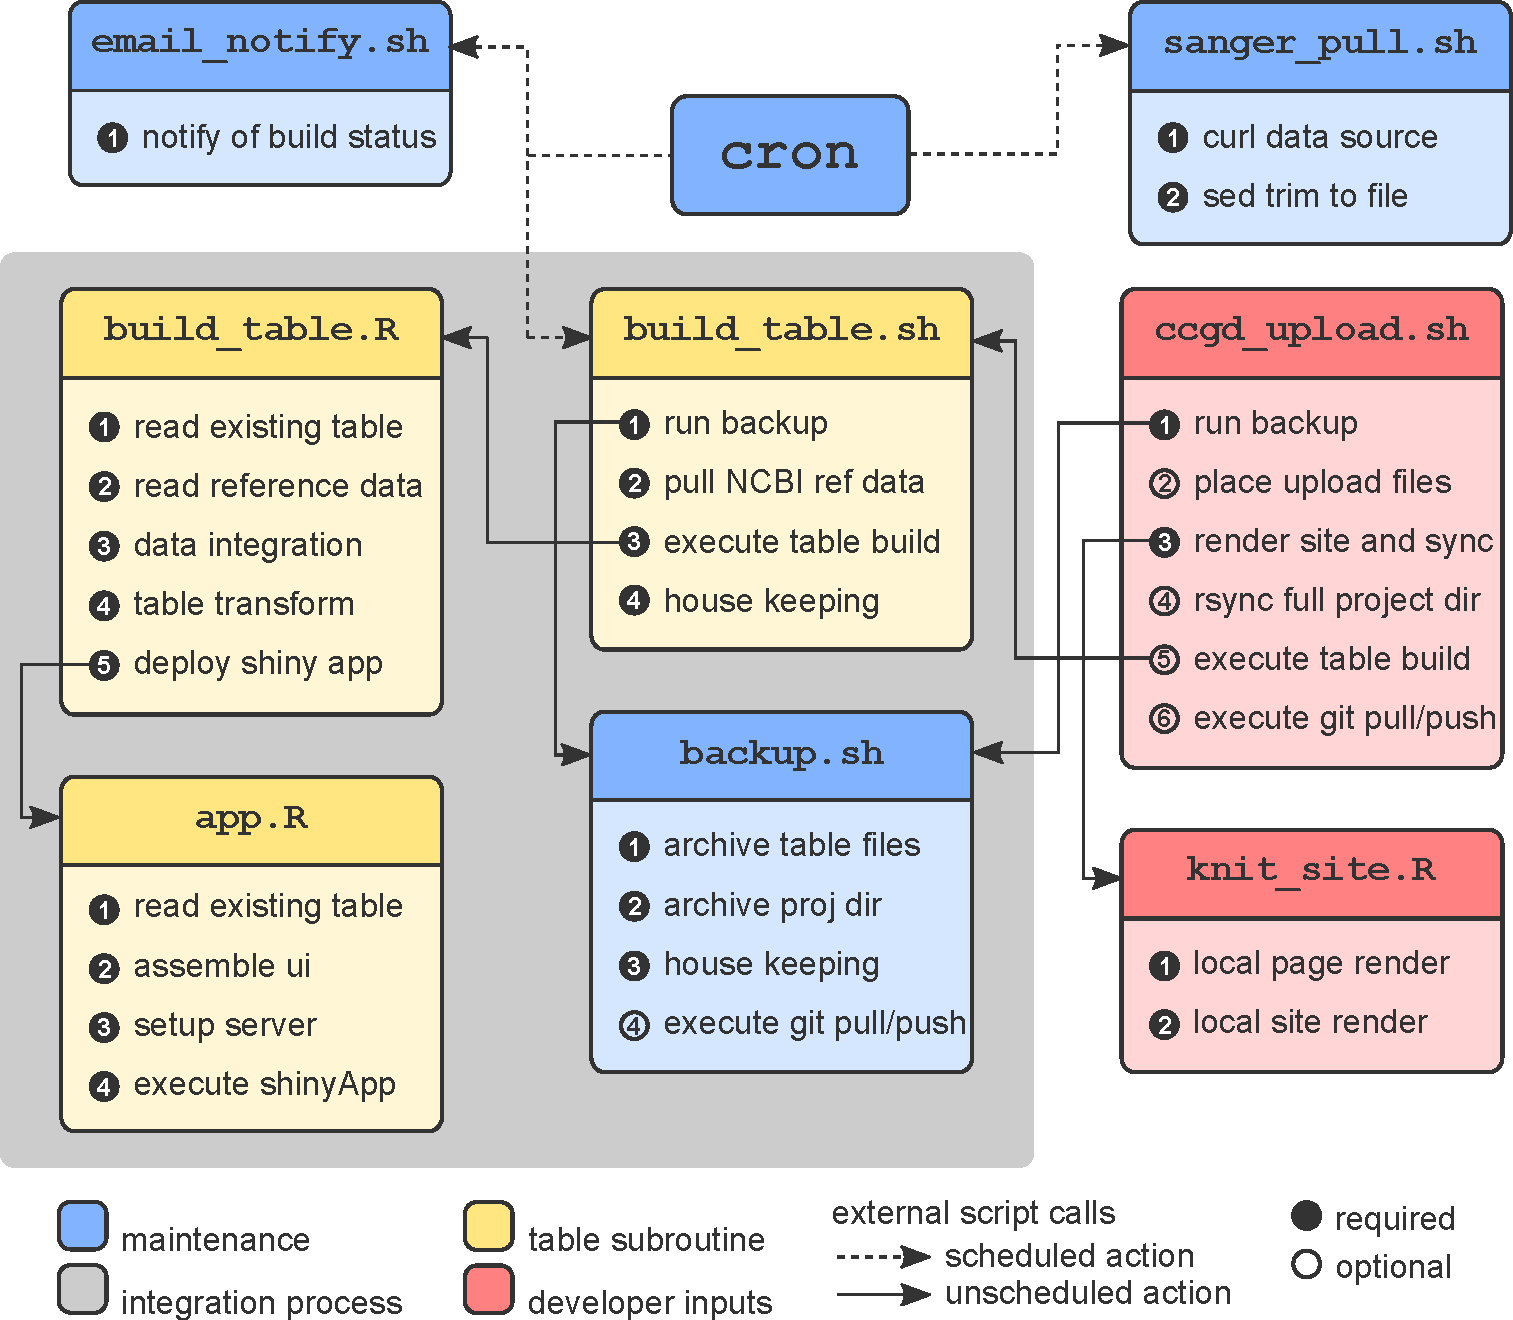
\includegraphics[width=0.8\textwidth]{fig/subroutine_flow.pdf}
    \caption[Subroutine flow]{\textbf{Subroutine flow} This diagram offers an overview of the actions and relationships within the executable scripts of the CCGD\@. Prior functionality was more effectively delineated into subroutines for better modularity. Also shown is the added functionality brought by the rebuilt data integration process. A hallmark of the difference between this new and old process is the use of R and shiny as the central frameworks to build the table as implemented in the \texttt{build\_table.R} and \texttt{app.R} scripts. It can also be seen that the integration process is automated by the system with a cron job among other maintenance tasks. Last, the \texttt{ccgd\_upload.sh} and \texttt{knit\_site.R} scripts were created to allow for introduction of new table data or the manual execution of any of the app subroutines.}\label{fig:subroutine}
\end{figure}

\subsection{Rshiny App}
In order to replace the existing CCGD search functionality our group employed the Rshiny framework. Simply put, the shiny app that now enables this central purpose is an interactive web interface for a single table. Several changes were made to the existing integration pipeline in order to achieve this simplicity.

The structure of a general shiny app follows a highly reduced and consistent paradigm, and ours is no different. The broad format of this work flow is \texttt{ui + server $\rightarrow$ deployment}. The server specifically has a discrete composition made up of reactive constructs of inputs, expressions, and outputs that shape the app's reactive graph, which forms, more accurately, the discrete operation of the application. The assembly and movement of this graph is both emblematic and practical in displaying the modularity and improved resource utilization of the reactive elements. Without belaboring the description of reactive programming, this model employs a declarative programming style that allows for lazy code execution~\cite{wickhamMasteringShinyBook}. What this amounts to in application is for the developer to define loose controls at a higher level while allowing the code to passively fill these requirements. This translates to greater flexibility to both the developer and the machine as resource use can be reduced through modularity in code execution.

\begin{figure}[H]
    \center{}
    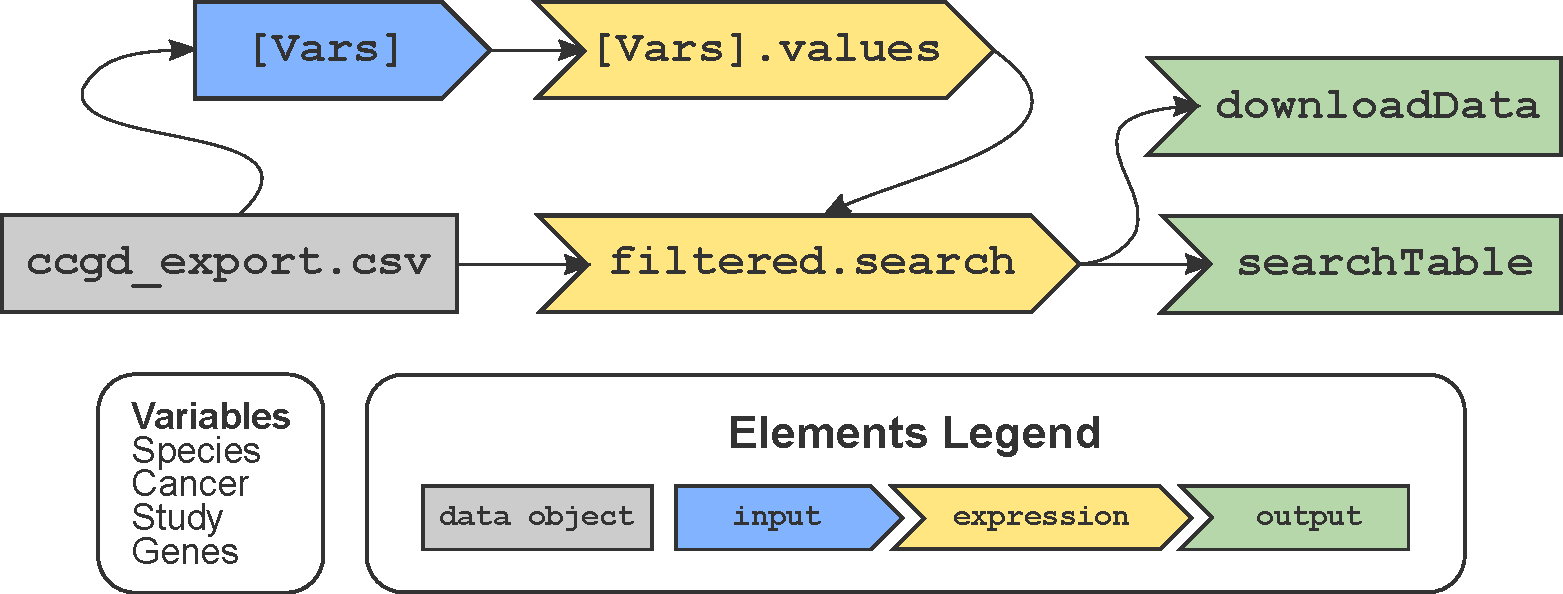
\includegraphics[width=0.8\textwidth]{fig/reactive_graph.pdf}
    \caption[\texttt{table\_app/app.R} Reactive Graph]{\textbf{\texttt{table\_app/app.R} Reactive Graph} An Rshiny app design can be defined by its reactive graph. The graph above displays the process flow of our app by highlighting modularity in the data streams around the table filtering process. The reactive web design is intended to allow for the automatic implementation of changed states applied through the alternate paths of the graph. This allows for the passive display of a static representation of the table while allowing for dynamic adjustment to filtering inputs through the \texttt{[Var] $\rightarrow$ [Var].values} path. Additionally, this declarative model provides for an interactive table array while only drawing computation when the appropriate event is called.}\label{fig:reactiveGraph}
\end{figure}

Within the scope of the \href{https://github.com/ctastad/ccgd/blob/master/table_app/app.R}{\texttt{table\_app/app.R}} server function we had a relatively simple goal of defining variable filters across the CCGD data table. Taking advantage of Rshiny's modularity, we created a two state path for the imported data object that allowed for both a variable-specific filter step along with a static, unchanged display of the table (see Figure~\ref{fig:reactiveGraph}). The advantage in doing this is that the table is displayed immediately on page load without the need to initiate a query. Additionally, the full, unfiltered table is available from the \texttt{downloadData} output at this state as well. For processing going down the filtered path, independent variable inputs are available to the user which are passed through two expression elements. In selecting a variable filter the \texttt{[Vars].values} expression applies a syntactic subsetting of the variable's data list which is then past to the central \texttt{filter.search} where the broader subsetting is carried to the rest of the table. The \texttt{searchTable} function takes the output of the filter and applies several text mutations to add external linking to several associated resources.

A small but fundamental element of our shiny app design was the use of the \texttt{renderDataTable} function in generating the \texttt{searchTable} output. The prior iteration of the CCGD architecture employed a relatively disproportionate Structured Query Language (SQL) database to store and serve numerous component elements that made up the table. Instead, the new implementation of our app now leverages the server-side processing capability of the DataTables JavaScript library. More specifically, we set parameters to create a reactive version of our function which allows for paging, searching, filtering, and sorting in real-time within the shiny server infrastructure [citeme DataTables]. Through this function alone we established new server paradigm that eliminated the SQL database.

\begin{figure}[H]
    \center{}
    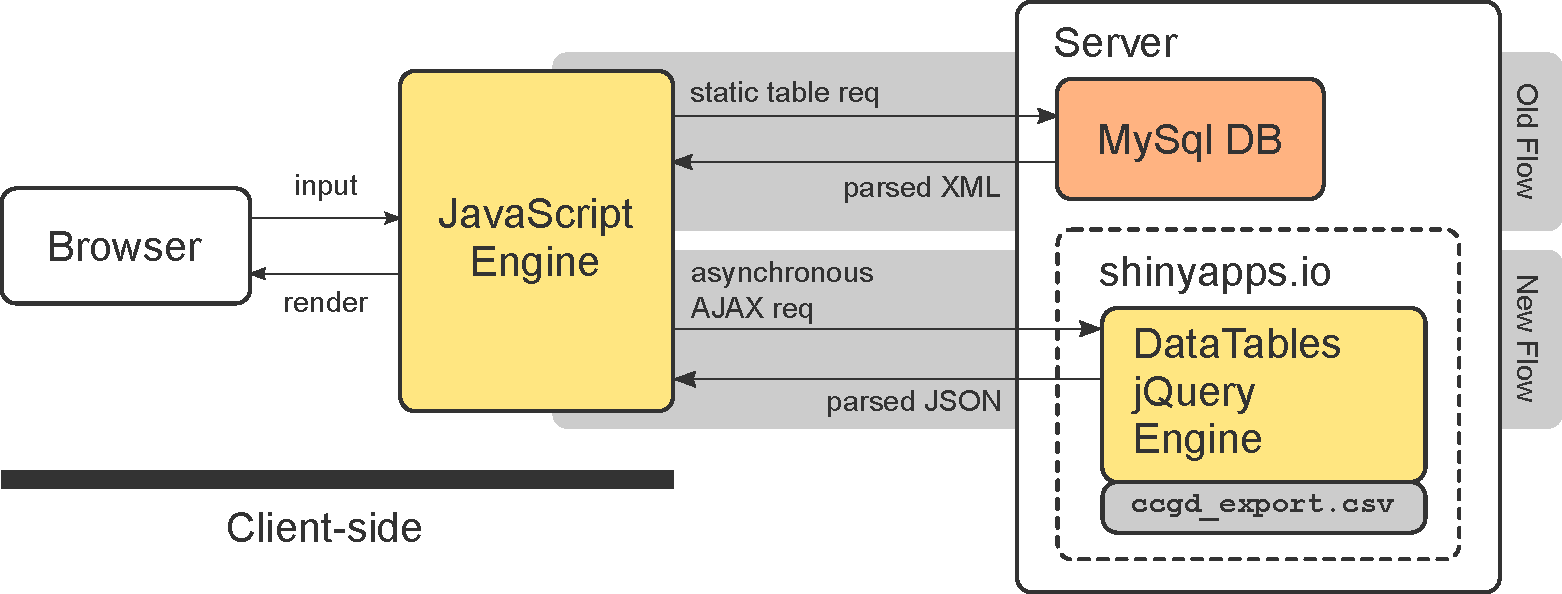
\includegraphics[width=0.8\textwidth]{fig/parse_flow.pdf}
    \caption[Server-side Processing Flow]{\textbf{Server-side Processing Flow} This diagram illustrates a small but fundamental change applied to the application table processing through the lens of the server-client relationship. The ``old'' flow shows the prior table processing procedure, which is highly typical of a classic Linux-Apache-MySQL-PHP (LAMP) stack website. Inputs and calls made by the browser occur from and within a client-side rendering engine which delivers a static request to the server-side SQL database. The database returns content parsed in Extensible Markup Language (XML) to the browser that is rendered and displayed. Our fundamental shift was to move this data processing entirely to JavaScript. Typically, this would result in client-side processing that would prohibit large tables like ours. Instead, we leveraged a server-side engine to handle Asynchronous JavaScript and XML (AJAX) requests which are returned with parsed JavaScript Object Notation (JSON), shown in the ``new'' flow. This processing flow allows for the use of a single~.csv file as the data source in table presentation, ordering, and pagination, ultimately eliminating the need for a SQL architecture.}\label{fig:parseFlow}
\end{figure}

\subsection{Best Practices}
Some features of the software best practices from the previous version of the CCGD were done quite well such as the level of detail in the documentation. At the same time, many other important areas were missing in the development and maintenance of the application. Most prominent among these were the lack of any degree of version control and relatively inconsistent design principles. As a result, our group employed or improved upon several methods in an effort to elevate the quality, usability, and portability of our codebase and application~\cite{finchamSoftwareDevelopmentPractices2011}.

Throughout the course of the project we utilized a private github code repository for hosting and change tracking. This work has since been published on a public repository and assigned a DOI number through \href{https://zenodo.org/record/4422027}{Zenodo}. Furthering the spirit of project integrity, we expanded on the nature of the documentation for the user and, more prominently, the product owner. Specifically, documentation that was previously written in a Microsoft Word file was now recreated in markdown, and a notable tone and detail shift was made in serving the information portability between administrators.

In approaching the process of development, we applied a philosophy of tidy code creation to both syntax and design. A supporting method in creating a more elegant code syntax was the use of R universe tools, Tidyverse and Rmarkdown. Both offer a coding grammar that is centered around accessibility and simplification of high-level language organization~\cite{wickhamWelcomeTidyverse2019}. Furthering this simplification, we sought opportunities to deduplicate and extract subroutines in the table integration process in an effort to streamline resource constraints. Finally, another notable area for improvement we sought was in disk space utilization. The existing integration process relied on the continuous presence of what were several intermediary files that occupied a sizable disk capacity. To combat this we specifically reworked several data transformation steps to allow for the post-process elimination of these temporary data objects.

\section{Results}

\subsection{Architecture Upgrades}
Following the goals set out in our project requirements, we chose Rmarkdown as a replacement framework to develop the application's web front-end. Previously, the web interface for the application had been developed using Adobe Dreamweaver~\cite{abbottCandidateCancerGene2015a} resting on a traditional LAMP stack. For the time, a LAMP stack and Dreamweaver served the purpose of simplifying the process of interface construction on a stable and consistent web platform, yet we hoped to extend the theme of simplified content creation into a modern framework. Further, utilizing a language such as Rmarkdown almost fully carries the development process into a state of pure content creation. Through the Rmarkdown toolset, the work of web design is now largely rendered automatically for the developer (see Figure~\ref{fig:renderFlow}). Employing the R web scheme established a cornerstone for the project to leverage both enhanced web development as well as making available other key tools in architecture design choices.

Continuing with those architecture choices, Rshiny stood as a natural segue from the Rmarkdown front-end to assemble the table application itself. By upgrading the web paradigm from that LAMP stack used in the prior version, we were able to shed some of the burden that come with that classic architecture in creating the new table application. This was further realized by leveraging the Rshiny toolkit. A central premise of the Rshiny design philosophy promotes interactive or reactive web applications (see Figure~\ref{fig:reactiveGraph}). With that philosophy comes a set of nimble features that are flexible, lightweight, and, still, very powerful. Taken together, refactoring the table in Rshiny code allowed us to fully replace the functionality of a SQL-based table with a JavaScript-powered backend that conducts previously resources intensive tasks in real-time (see Figure~\ref{fig:parseFlow}). This is all furthered by the fact that the dramatically improved ease of development found in Rmarkdown, largely carries into Rshiny as well.

\subsection{Design Changes}
The foundation laid by these architecture changes provided many substantive avenues for improved design. Following best practices as well we also developed improved workflows which extended those core structural improvements. The most substantive of these gains was found in the complete rebuild performed on the data integration process. Given that we established a new framework built on R, it was necessary to extend modifications to the length of the full pipeline. In doing so, we also explored improvements in the base process peripheral to the new R code as there were opportunities to improve these workflows. As a result, we broke several existing functions into dedicated subroutines for improved modularity in both script execution and data management. Additionally, the considerations given to redesigning these script functions led to the development of improved app inputs in the form of more accessible manual controls. The convergence of the advances made in these design choices is maybe best illustrated by the site render function. A functionality newly created, the \texttt{knit\_site.R} script was only made possible through the features and ease of the Rmarkdown architecture. The effort to package this process as a subroutine elevated these mechanisms to the level of being a component of the application rather than just actions performed to conduct development (see Figure~\ref{fig:subroutine}).

Along with software design changes, there were several improvements made to the interface and site appearance. The upgraded web front-end not only offered a needed facelift to the aesthetic appearance of the site, but the new framework brought many of the elements of the page construction current with existing browser standards. While not an original goal established in our project requirements, the many considerations that go into web element compatibility are well served in this update, ultimately reducing risk of unintended obsolescence. Minor usability factors were considered as well such as the creation of an improved URL\@. The CCGD can now be accessed via~\href{https://z.umn.edu/ccgd}{(z.umn.edu/ccgd)} rather than the much more unruly~\href{http://hst-ccgd-prd-web.oit.umn.edu/}{(http://hst-ccgd-prd-web.oit.umn.edu/)}. A more major usability achievement was derived from the structure of the new Rshiny table interface. With the combination of the reorganized data integration process, the elimination of the SQL backend, and the front-end chosen in the DataTables library, we were able to assemble the application as a single page. This dramatically reduced broader site map complexity and simplified the process of interacting with the same data set for the user overall.

\subsection{Resource Use Improvements}
Special consideration was given to resource use throughout the refactoring process. Generally as a measure of best practice, resource improvements were sought at all times within engineering deliberation. Still, a more concrete issue was present with the recent development of space constraints in the existing production version shortly prior to the project start. We sought ways to most effectively address this acute issue in the existing design and identified several persistent data files as notable offenders of disk use. Notably, several large reference files in the data integration process were being written to disk. We assessed these files and identified several candidates for house keeping integration post-process and found ways to compress those that need remain persistent. This alone generated approximately a 50\% reduction in existing space use. Further dramatic space reduction was realized with the elimination of the SQL database. All together, these combined changes took a server instance that sat at approximately 23GB and brought it to 150MB\@ (see Figure~\ref{fig:spaceTree}).

Another broad concept we addressed in elevating general efficiency was exploring general concepts of technical debt. This idea is addressed in our approach to dealing with space constraints on some level, but it is a problem that can generally permeate an entire codebase. An effective illustration of this is given by the qualitative view of the total file tree present in the site directory (see Figure~\ref{fig:fileTree}). It can be difficult to pin point the driving factor in what leads to the accumulation of software entropy, but it is easy to see it exists nonetheless. By continuing our emphasis on best practices, we were able to leverage the simplified architecture upgrades alongside elimination of some functional redundancy to generate a working code base that spans across a much more tidy tree.

\begin{figure}[H]
    \center{}
    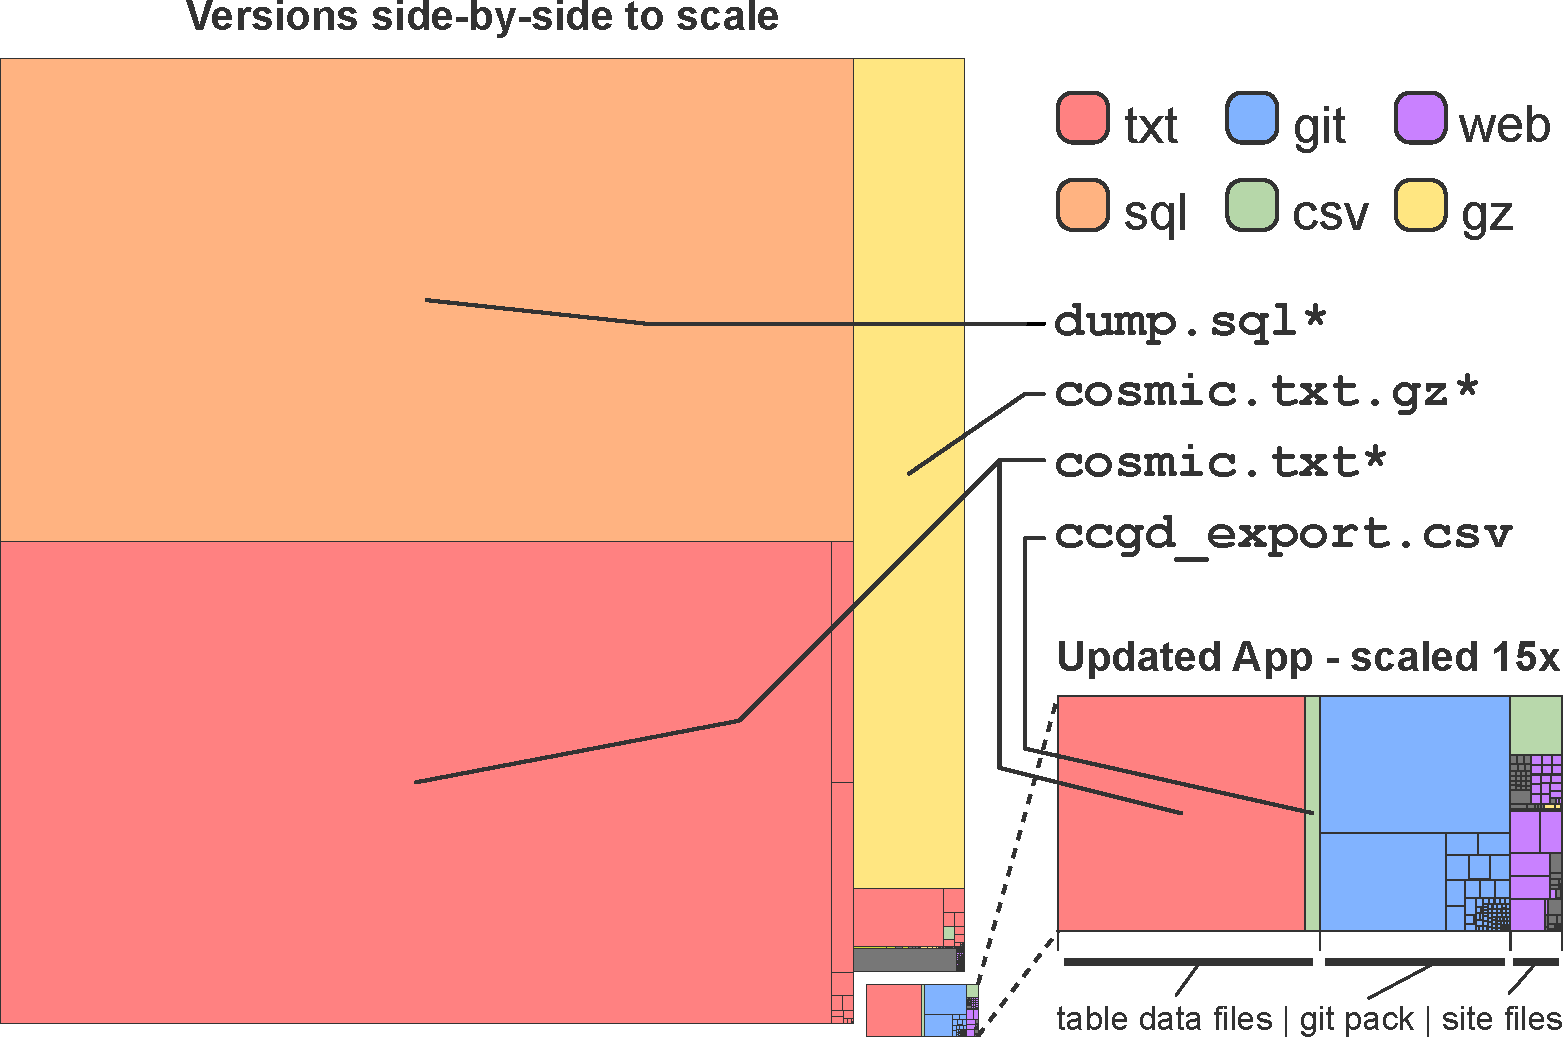
\includegraphics[width=0.8\textwidth]{fig/space_tree.pdf}
    \caption[Disk Use Comparison]{\textbf{Disk Use Comparison} shows a treemap which illustrates the substantial difference in disk utilization between CCGD versions. The original to-scale map on the left gives an exploded view distinguishing the updated app treemap in the bottom right corner with all remaining elements of the map belonging to the old version. This visual comparison emphasizes the [10x] space decrease made during the upgrade. The fruits of several design choices are present in this space reduction. The most notable impacts of these choices are several massive files eliminated or substantially reduced (noted by asterisk). Notably, the dump.sql file shown represented the disproportionate size of the database and space payoff earned by eliminating it. Also, it can be seen that the persistent cosmic.txt data file is present in both versions. Improvements made in post-process trimming of files like this also produced substantial space returns. Last, the rebuilt table build process transitioned several data objects shown from persistent to transient.}\label{fig:spaceTree}
\end{figure}

Ref crossdirstat

\begin{figure}[H]
    \center{}
    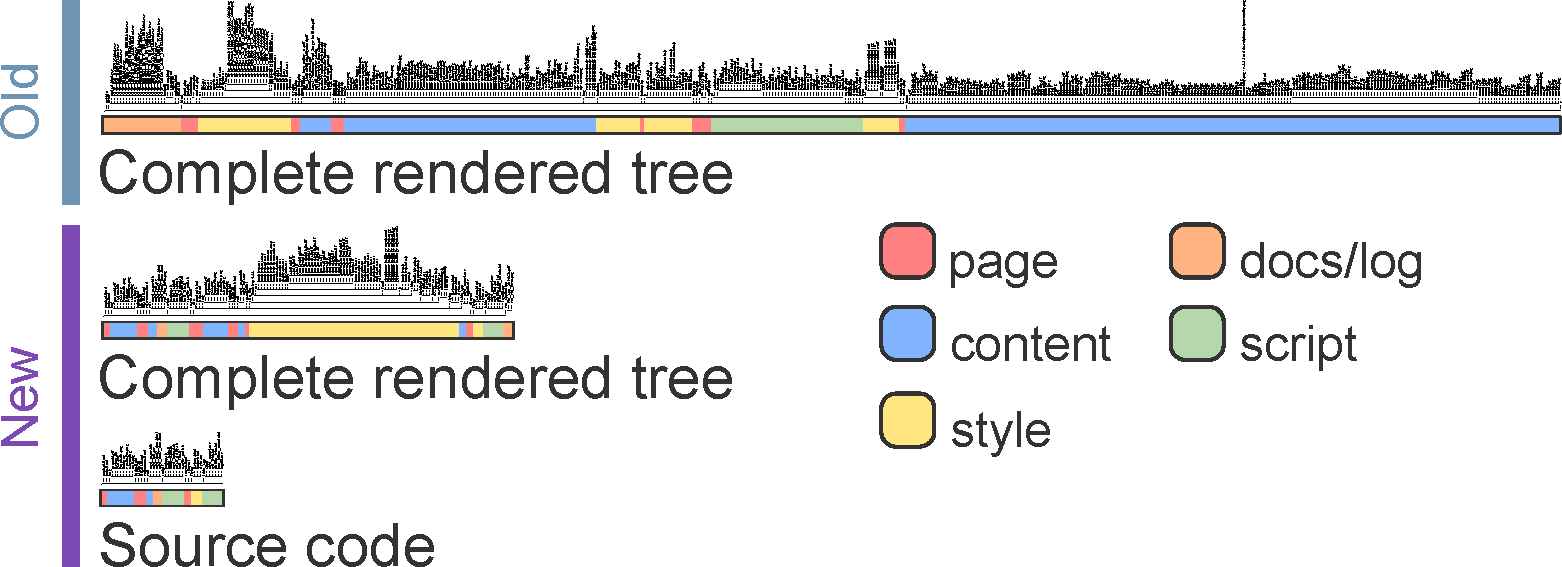
\includegraphics[width=0.8\textwidth]{fig/file_tree.pdf}
    \caption[Project Directory File Tree Comparison]{\textbf{Project Directory File Tree Comparison} The above figure offers a qualitative assessment of an element of technical debt that was improved in refactoring. Shown are the horizontally oriented file trees of the site directories of the new and old projects. What is illustrated is a dramatic improvement in the tree size and complexity through the elimination of a large degree of redundant or unnecessary content, log, and style files. This is accentuated even further when comparing the source code. This was accomplished both in the intentional design of eliminating content redundancy and in the streamlined structure of the Rmarkdown rendering process. This allowed for the elimination of several dimensions of broader web design and table build data elements.}\label{fig:fileTree}
\end{figure}


\begin{figure}[H]
    \center{}
    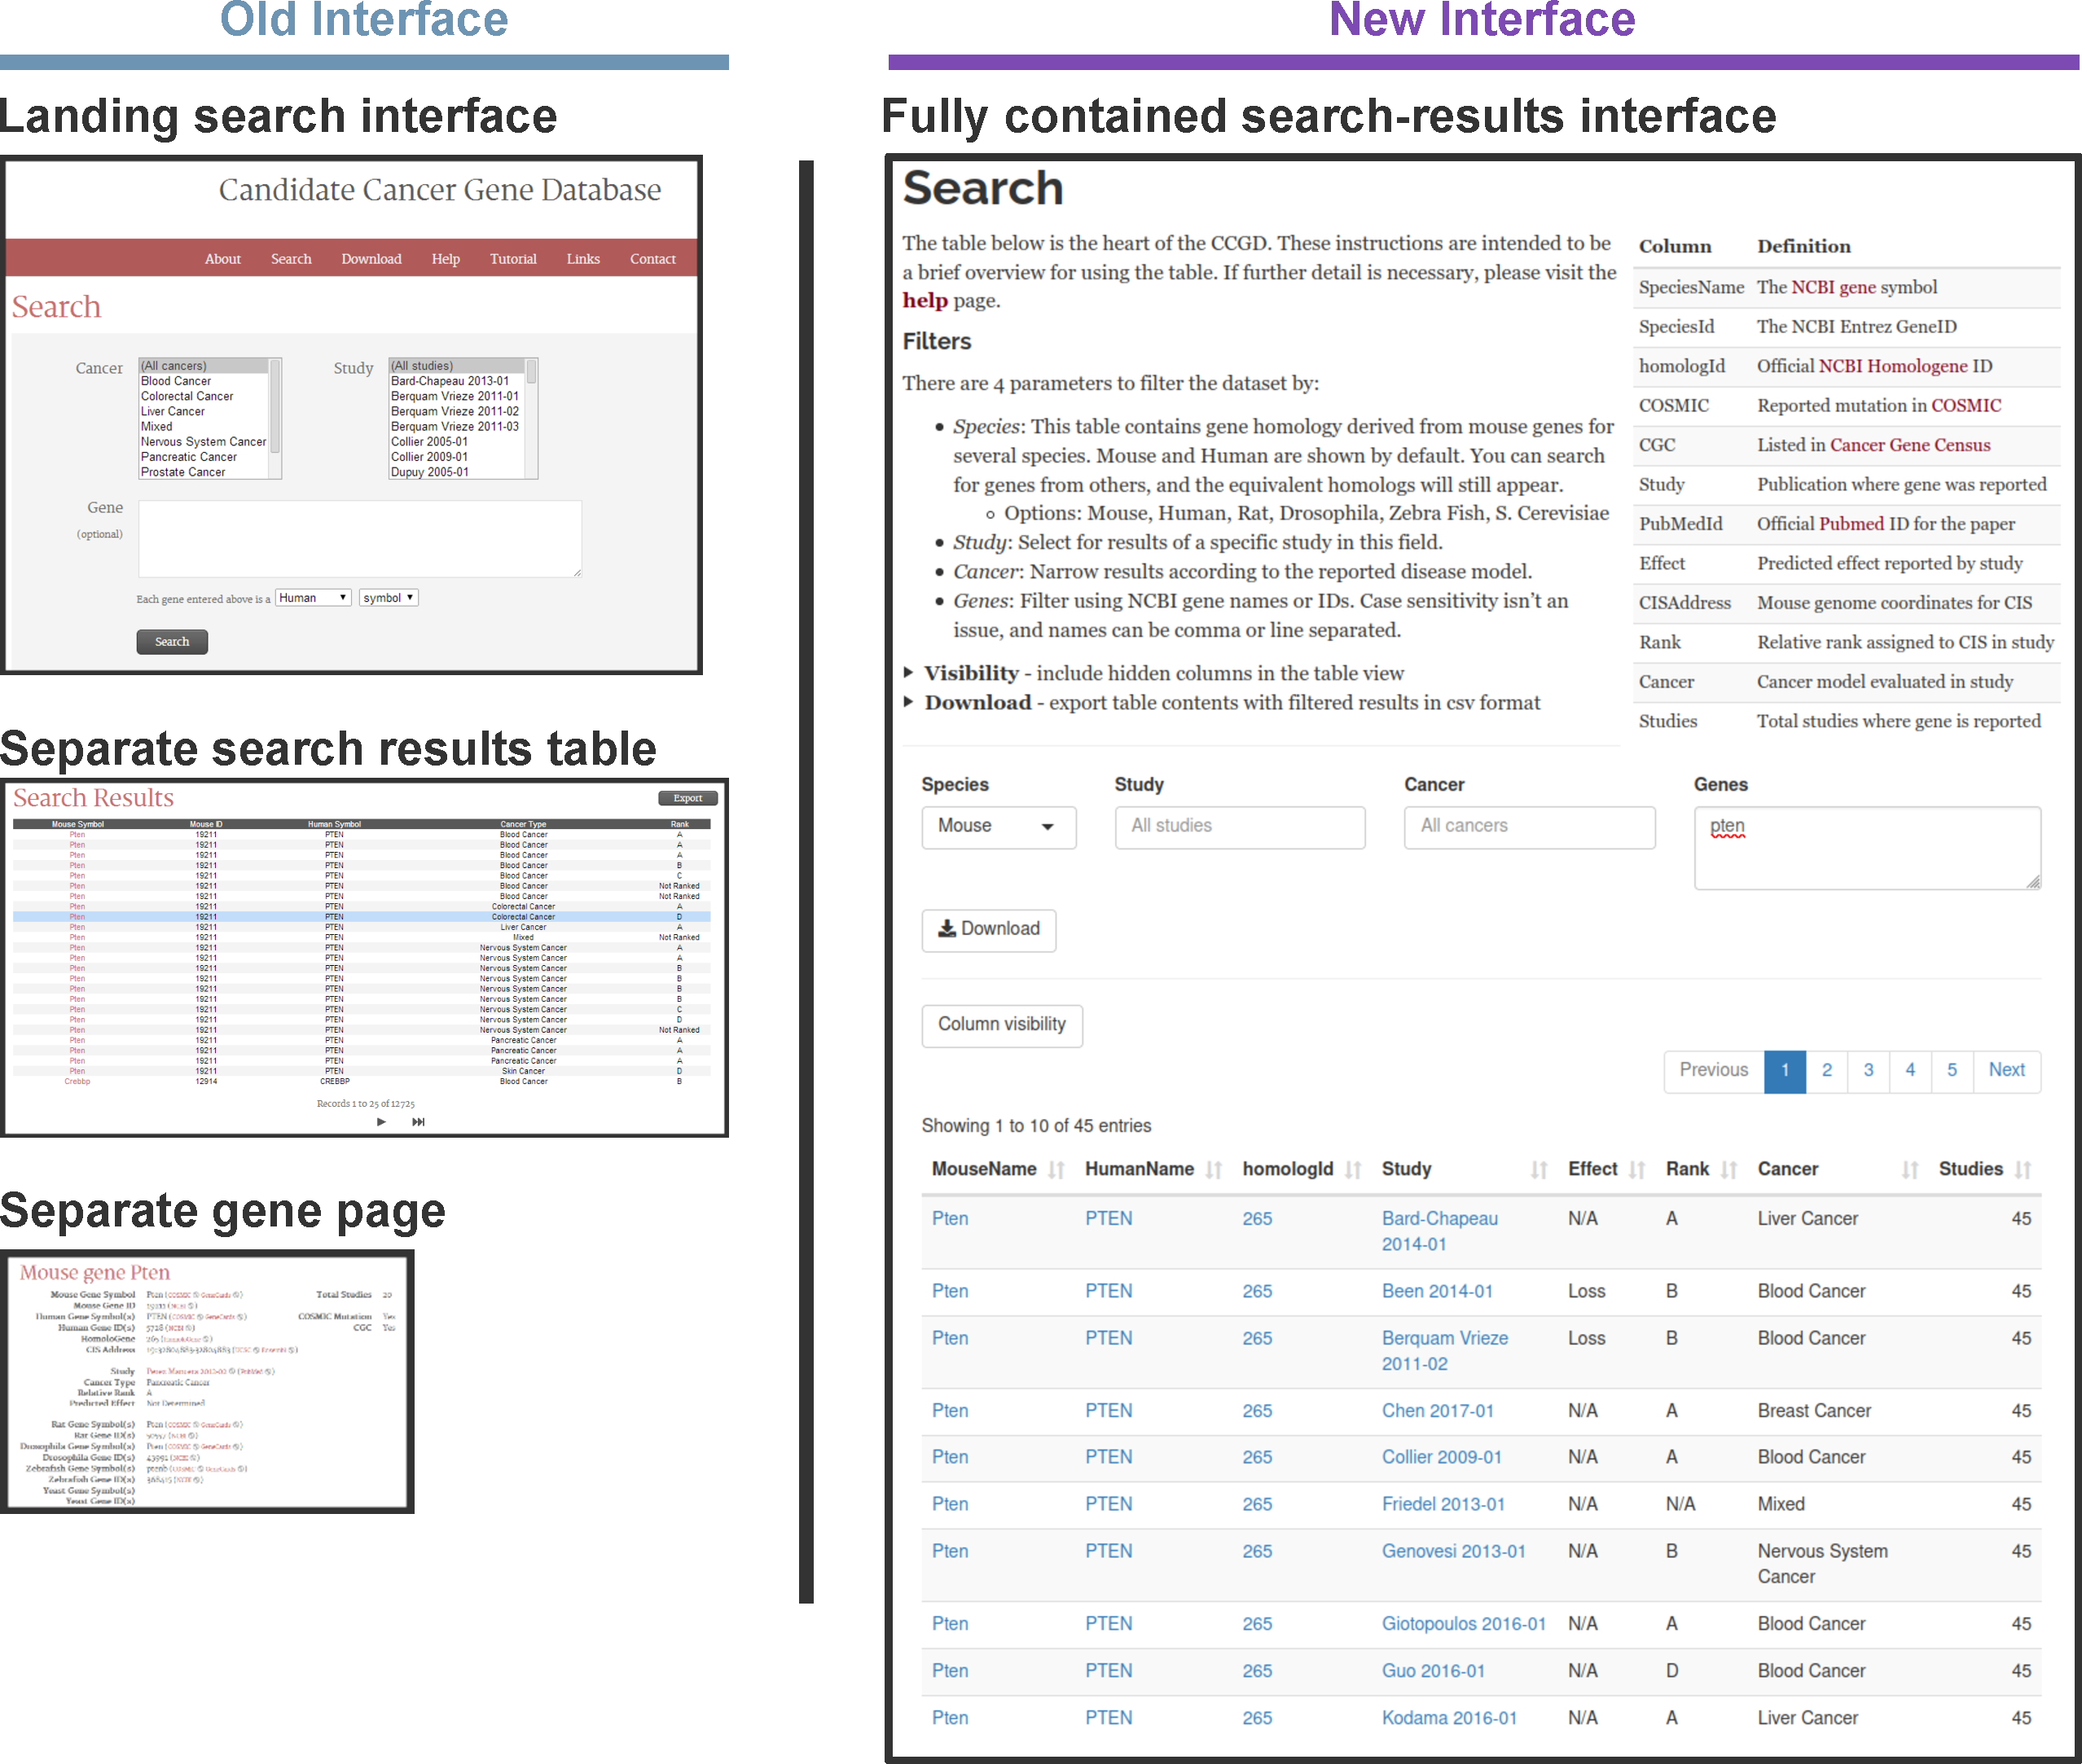
\includegraphics[width=0.8\textwidth]{fig/interface.pdf}
    \caption[Search Interface Changes]{\textbf{Search Interface Changes}}\label{fig:interface}
\end{figure}
%%%%%%%%%%%%%%%%%%%%%%%%%%%%%%%%%%%%%%%%%%%%%%%%%%%%%%%%%%%%%%%%%%%%%%%%%%%%%%%%

% Conclusions

%%%%%%%%%%%%%%%%%%%%%%%%%%%%%%%%%%%%%%%%%%%%%%%%%%%%%%%%%%%%%%%%%%%%%%%%%%%%%%%%

\chapter{Conclusions}
This work has given new life to the CCGD and the valuable functionality that it offers in the form of accessible forward genetic cancer screen data. Further, it has been a case study in the benefits of evolving of tool sets and frameworks that increasingly live at the nexus of the field of Bioinformatics. We've given a general characterization of the contrast that can exist between development schemas that are separated by only 5 years time and the substantive impact to be had in adopting these new paradigms.

With that, the CCGD will continue to function as it has since its initial release by offering a point of integration for collated results in the cancer gene screening space. Existing connections have been maintained both to and from external resources such as those from the CCGD pointing to the GeneCards suite, NCBI's HomoloGene, and any associated screening publication. Additionally, an external gene-level reference link pointing to the CCGD from the Sanger COSMIC database has been maintained as well. Finally, new studies will continue to be integrated into the core table as they are published and curated, as was done before.

Finally, we have maintained the essence of that functionality while notably reducing the digital entropy within the codebase and application architecture. At the heart of this redesign, we have placed the Rmarkdown web paradigm at the center of the application. We feel this offers not only an expanded repertoire of functionality and features but brings the application stack to parity with many of the comparable Bioinformatics web tools of the day. In doing so, we implemented our design with an elevated consideration for best practices in development resulting in improved resource outcomes and overall performance. This is reflected by qualitative and quantitative comparisons of the codebase. We also placed added focus on the nature of the documentation and portability of the code, which is now publicly hosted under the open-source MIT license at github (https://github.com/ctastad/ccgd), (https://doi.org/10.5281/zenodo.4422026). With this approach, we hope that the sustained service of the CCGD will continue to serve the research community at-large now and for future refactorizations yet to come.

\addcontentsline{toc}{chapter}{Bibliography}
\printbibliography{}

\end{document}
